% ****** Start of file apssamp.tex ******
%
%   This file is part of the APS files in the REVTeX 4.2 distribution.
%   Version 4.2a of REVTeX, December 2014
%
%   Copyright (c) 2014 The American Physical Society.
%
%   See the REVTeX 4 README file for restrictions and more information.
%
% TeX'ing this file requires that you have AMS-LaTeX 2.0 installed
% as well as the rest of the prerequisites for REVTeX 4.2
%
% See the REVTeX 4 README file
% It also requires running BibTeX. The commands are as follows:
%
%  1)  latex apssamp.tex
%  2)  bibtex apssamp
%  3)  latex apssamp.tex
%  4)  latex apssamp.tex
%
\documentclass[%
 reprint,
%superscriptaddress,
%groupedaddress,
%unsortedaddress,
%runinaddress,
%frontmatterverbose, 
%preprint,
%preprintnumbers,
%nofootinbib,
%nobibnotes,
%bibnotes,
 amsmath,amssymb,
 aps,
%pra,
%prb,
%rmp,
%prstab,
%prstper,
%floatfix,
]{revtex4-2}
\usepackage{kotex}
\usepackage{graphicx}% Include figure files
\usepackage{dcolumn}% Align table columns on decimal point
\usepackage{bm}% bold math
%\usepackage{hyperref}% add hypertext capabilities
%\usepackage[mathlines]{lineno}% Enable numbering of text and display math
%\linenumbers\relax % Commence numbering lines

%\usepackage[showframe,%Uncomment any one of the following lines to test 
%%scale=0.7, marginratio={1:1, 2:3}, ignoreall,% default settings
%%text={7in,10in},centering,
%%margin=1.5in,
%%total={6.5in,8.75in}, top=1.2in, left=0.9in, includefoot,
%%height=10in,a5paper,hmargin={3cm,0.8in},
%]{geometry}

\def\rcurs{{\mbox{$\resizebox{.16in}{.08in}{
\includegraphics{ScriptR}}$}}}
\def\brcurs{{\mbox{$\resizebox{.16in}{.08in}{
\includegraphics{BoldR}}$}}}
\def\hrcurs{{\mbox{$\hat \brcurs$}}}

\begin{document}


\title{약산의 적정과 분리 실험 결과보고서}

\author{서울대학교 전기정보공학부 2018-12432 박정현}
 \email{alexist@snu.ac.kr}
\date{\today}% It is always \today, today,
             %  but any date may be explicitly specified

\begin{abstract}
abdcd
\end{abstract}

%\keywords{Suggested keywords}%Use showkeys class option if keyword
                              %display desired
\maketitle

%\tableofcontents

\section{\label{sec:level1}Assignment}
\subsection{\label{sec:level2}Problem1}
\subsection{\label{sec:level2}Problem2}


\section{\label{sec:level1}Introduction}
\subsection{\label{sec:level2}$NaOH$표준화}
$KHP$와 $NaOH$ 화학 반응식은 아래와 같다.
\begin{align}
	NaOH + KHC_{8}H_{4}O_{4} &\rightarrow KNaC_{8}H_{4}O_{4} + H_{2}O
\end{align}
본 실험에서 사용된 표준 용액은 $KHC_{8}H_{4}O_{4}$ $6mM$이다. 이 때 당량점에서 아래의 식이 성립한다. 이 때 위의 반응식에서 각각 하나의 $H^{+}$, $OH^{-}$가 반응하게 되므로 $n_{KHP}$, $n_{NaOH}$의 값은 $1$이다.
\begin{align}
	n_{KHP}M_{KHP}V_{KHP} &= n_{NaOH}M_{NaOH}V_{NaOH}\\
	V_{NaOH} &= \frac{M_{KHP}V_{KHP}}{M_{NaOH}}
\end{align}
이때 증류수 바탕적정에 투입된 $NaOH$의 양을 뺀 뒤 사용된 위의 식을 이용해 $NaOH$의 농도를 계산할 수 있다.


\subsection{\label{sec:level2}약산의 total acidity}
$CH_{3}(COOH)$, ($C_{6}H_{4}(OH)COOH$) 은 각 $pK_{a}=4.75$ [2], $pK_{a}=2.972$ [3]의 $pK_{a}$값을 가지며 $NaOH(aq)$와의 반응은 아래와 같다.

\begin{align}
	C_{7}H_{6}O_{3}(aq) \rightarrow C_{7}H_{5}O_{3}^{-}(aq) + H^{+}(aq) & pK_{a}=2.972\\
	C_{2}H_{4}O_{2}(aq) \rightarrow C_{2}H_{3}O_{2}^{-}(aq) + H^{+}(aq) & pK_{a}=4.75
\end{align}

따라서 total acidity에 대해서 아래의 식이 성립한다. 단, $M_{H^{+}}$는 약산이 모두 반응하는 총 몰수를 부피로 나눈 몰농도이다.

\begin{align}
	M_{H^{+}}V_{acid} &= V_{NaOH}M_{NaOH} \label{eq:total_acid}
\end{align}

\section{\label{sec:level1}Data and Results}
\subsection{\label{sec:level2}$NaOH$표준화}
$KHP$용액을 적정한 결과는 아래와 같다. 단, Tab.\ref{tab:NaOH_KHP}에서 오차는 최소 눈금으로 인한 오차이다. 해당 데이터를 선형회귀하면 Fig.\ref{fig:NaOH_KHP}와 같다.
\begin{table}[]
\begin{tabular}{c|c} \hline \hline
$KHP$ 부피[$mL$] & $NaOH$ 부피[$mL$] \\ \hline
$0.1\pm0.01$ & $3.38 - 3.18 - 0.04 = 0.16\pm0.02$  \\ \hline
$0.5\pm0.01$ & $4.30 - 3.50 - 0.04 = 0.76\pm0.02$  \\ \hline
$0.5\pm0.01$ & $5.11-4.35 - 0.04 = 0.72\pm0.02$ \\  \hline \hline 
\end{tabular}
\caption{\label{tab:NaOH_KHP}측정된 화학 반응여부}
\end{table}

\begin{figure}[htbp]
	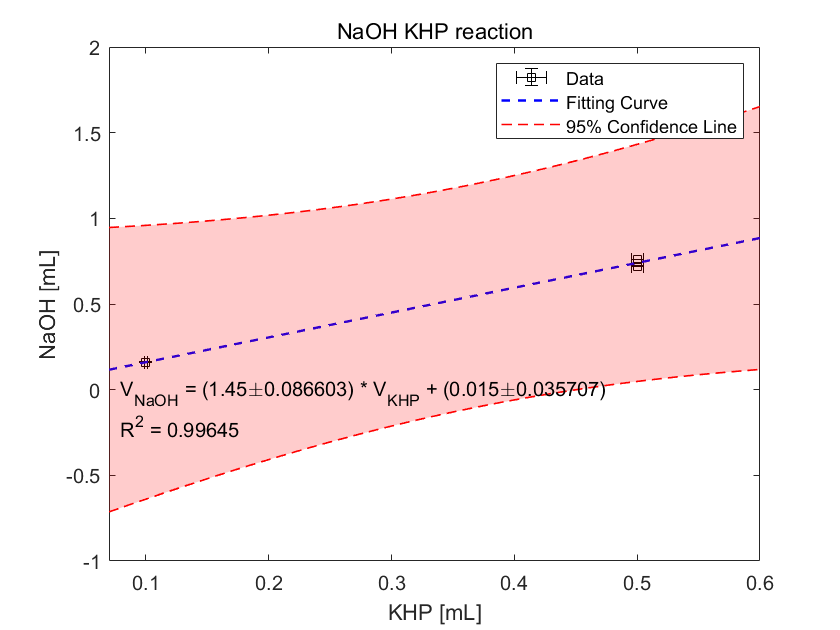
\includegraphics[width = 0.95\linewidth]{NaOH_KHP.png}% Here is how to import EPS art
	\caption{\label{fig:NaOH_KHP}$NaOH$, $KHP$ 반응부피에 대한 그래프}
\end{figure}
그래프의 기울기를 이용해 $NaOH$의 몰수를 계산하면 아래와 같다. 이 때 오차는 선형회귀 결과의 분산을 이용해 계산하였다.
\begin{align}
	M_{NaOH} &= 4.14 \pm 0.24 [mM]
\end{align}


\subsection{\label{sec:level2}약산의 total acidity}
약산의 혼합용액 $1.0mL$에 대해서 반응한 $NaOH$ 용액의 부피는 아래와 같다. 식 (\ref{eq:total_acid})을 이용했을 때 total acid는 아래와 같다. 단, 각각의 경우는 $NaOH$의 농도를 $1mM$로 둔 경우와 실제 측정된 $4.14mM$의 경우에 대해 계산한 결과이다.
\begin{align}
	V_{NaOH} &= (9.81 - 8.89) = 0.92 \pm 0.01 [mL]
\end{align}

\begin{table}[]
\begin{tabular}{c|c} \hline \hline
$M_{NaOH} = 1mM$ & $M_{NaOH} = 4.14mM$ \\ \hline
$0.92\pm0.01mmol$ & $3.80\pm0.04mmol$  \\ \hline
\end{tabular}
\caption{\label{tab:total acid}측정된 Total Acid}
\end{table}


\subsection{\label{sec:level2}약산의 분리}
C18카트리지를 $1mL$씩 밀며 적정했을 때 반응한 $NaOH$의 부피는 아래와 같다.
\begin{table}[]
\begin{tabular}{c|c} \hline \hline
이동 부피$\pm 0.01 [mL]$ & 반응한 $V_{NaOH} \pm0.01 [mL]$ \\ \hline
1 & $10.75-10.61 =0.14$\\ \hline
2 & $14.82-10.75=4.07$\\ \hline
3 & $16.48-14.82=1.66$\\ \hline
4 &$ 16.88-16.48=0.40$\\ \hline
5 &$ 17.00-16.90=0.10$\\ \hline
6 &$ 17.05-17.00=0.05$\\ \hline
7 &$ 17.15-17.05=0.10$\\ \hline
8 &$ 17.30-17.15=0.15$\\ \hline
9 &$ 17.40-17.30=0.10$\\ \hline
10 &$ 17.50-17.40=0.10$\\ \hline
11 &$ 17.60-17.50=0.10$\\ \hline
12 &$ 17.65-17.60=0.05$\\ \hline
13 &$ 17.72-17.65=0.07$\\ \hline
14 &$ 17.80-17.72=0.08$\\ \hline
15 &$ 17.85-17.80=0.05$\\ \hline
16 &$ 17.92-17.85=0.07$\\ \hline
17 &$ 18.10-18.00=0.10$\\ \hline
18 &$ 18.12-18.10=0.02$\\ \hline
19 &$ 18.20-18.12=0.08$\\ \hline
20 &$ 18.25-18.20=0.05$\\ \hline \hline
\end{tabular}
\caption{\label{tab:C18}크로마토그래피 후 각각의 적정 결과}
\end{table}

\section{\label{sec:level1}Reference}
[1] 김희준, \textit{일반화학 실험}(자유아카데미, 2016)\\

[2] D.W. Oxtoby, H.P. Gillis, and L. Butler, \textit{Principles of Modern Chemistry} (Brooks/Cole, Australia, 2020).

\end{document}
%
% ****** End of file apssamp.tex ******
